%%%%%%%%%%%%%%%%%%%%%%%%%%%%%%%%%%%%%%%%%%%%%%
%                insertmeeting
% 1) Title (something creative & funny?)
% 2) Date (MM/DD/YYYY)
% 3) Location (ex. Hagerty High School)
% 4) People/Committees Present 
% 5) Picture 
% 6) Start Time & Stop Time (ex. 12:30AM to 4:30PM)
%%%%%%%%%%%%%%%%%%%%%%%%%%%%%%%%%%%%%%%%%%%%%%
\insertmeeting 
	{First Field Test} 
	{10/12/21}
	{Hagerty High School}
	{Annika, Anouska, Clayton, Falon, James, Jensen, Nathan, Ritam, Rose, Samantha, Lilly}
	{Images/RobotPics/robot.jpg}
	{2:30 - 4:30}
	
\subsection*{General}
\noindent\hfil\rule{\textwidth}{.4pt}\hfil
\subsubsection*{Goals}
\begin{itemize}
    \item Practice driving tank robot
    \item Evaluate and fix issues 

\end{itemize} 

\noindent\hfil\rule{\textwidth}{.4pt}\hfil

\subsubsection*{Accomplishments}
At this team meeting, we did the first field test of our tank drive robot!  Before we got started however, our software team created a tele-op program. Instead of using standard tank controls, we decided to use arcade drive, where one stick controls tuning and the other controls speed. This will make our driving a bit smoother going around corners. With everything ready, we started driving the robot around the field, doing as many cycles as possible. We quickly found out that driver practice was going to be very important this year, especially because of our lack of experience. What we saw was that most of the time was spent going through the gap in the barriers and turning the corner to head towards the shipping hub (Figure \ref{fig:pic1}). Using the car drive should make this process a bit easier, but we came up with the idea to make some round parts that attach onto the corners that reduce damage from slamming against the wall, so we CADed and cut them, and attached them to the robot (Figure \ref{fig:pic2}). 
One other issue we faced was the robot dropping the block as we lifted the arm, a problem that slowed us down significantly. We came up with two separate ideas on how to fix this; one software, and one hardware. For the software solution we wanted to slow down the movement of the arm as it rotates upwards so that less force is exerted on the block. To do this, we came up with an equation for the position and speed of the arm and graphed it on a graphing calculator to ensure it was correct (Figure \ref{fig:pic3}. The hardware solution involved changing the grabber to hold the block more firmly. One way to do this is to move the servo mount forward so that the center of rotation is closer to the cargo we are trying to pick up. Moving the servo forward will also make the grabber shorter, so it won't get caught on the shipping hub, as we saw a few times during our testing.  Another way we planned to improve the hardware was to expand the width of the grabber, creating more friction on the block we are picking up, ensuring it doesn’t fall out before we open the grabber. We made all these changes in CAD, cut out all the parts on the glowforge, then attached it to the robot (Figure \ref{fig:pic4}). With all of these changes, we plan on testing them out in a future meeting.
 

\begin{figure}[ht]
\centering
\begin{minipage}[b]{.50\textwidth}
  \centering
  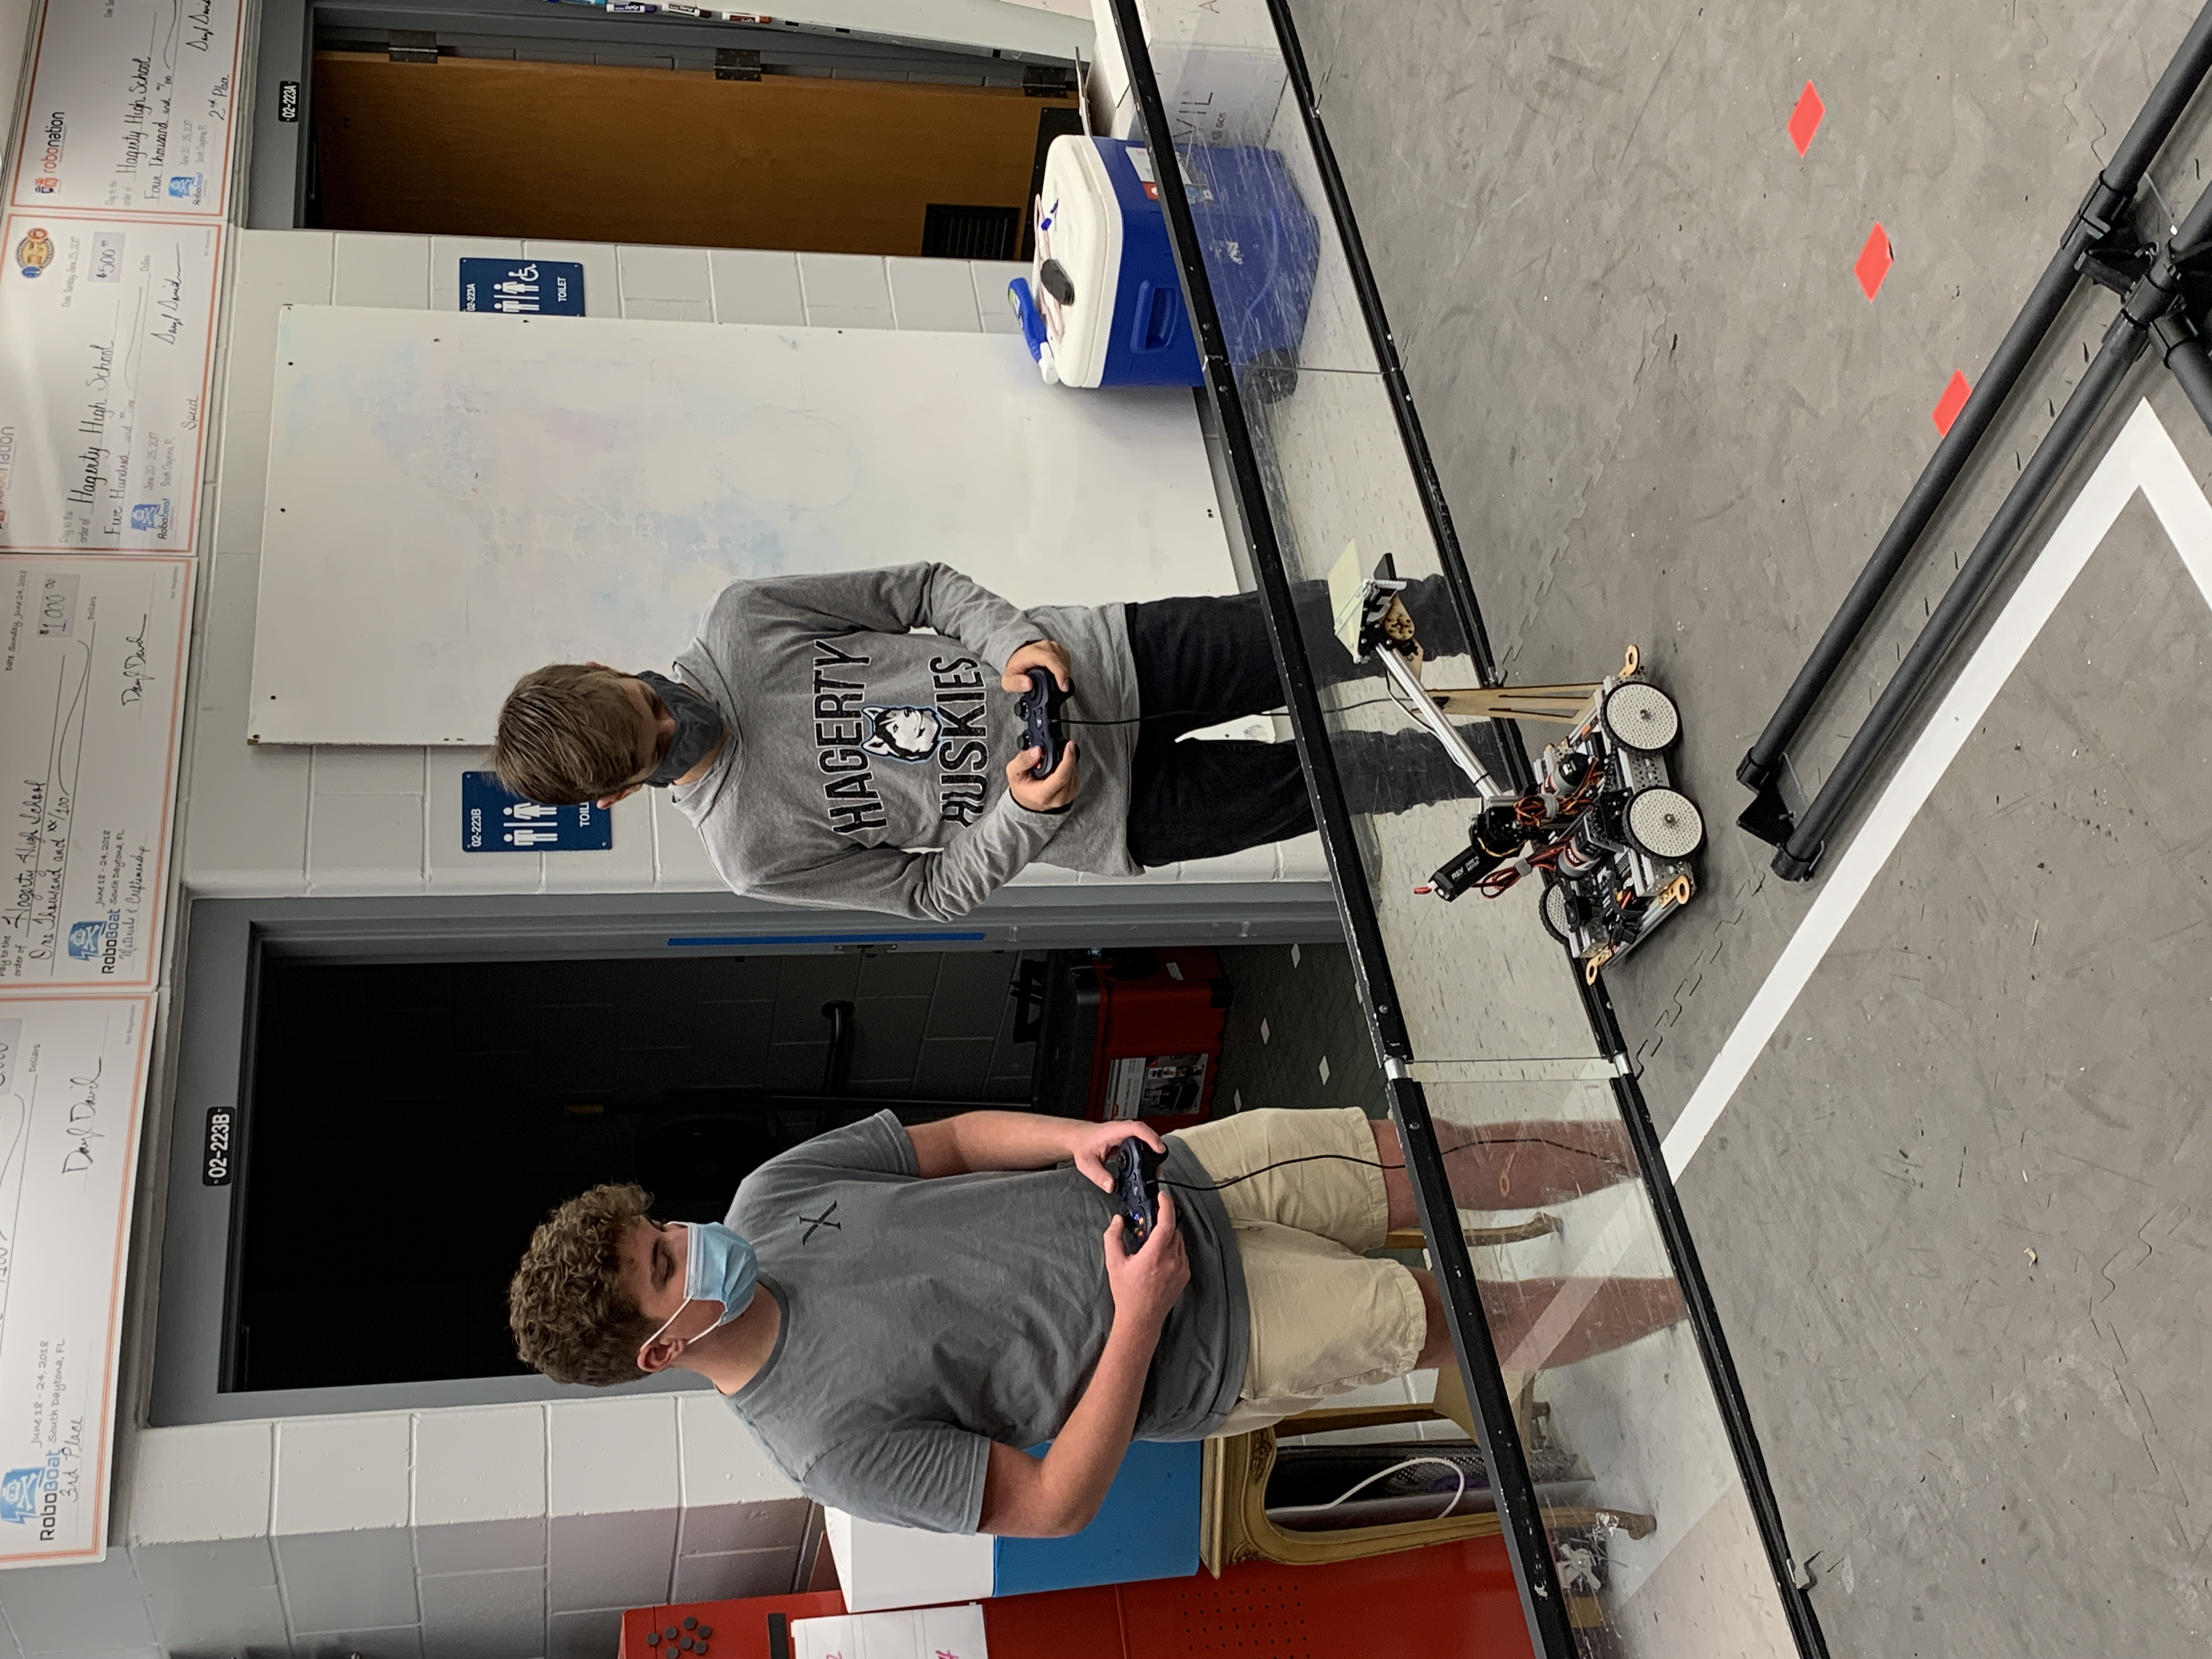
\includegraphics[width=0.8\textwidth]{Meetings/October/10-12-21/10-12-21_Team_Figure1 - Nathan Forrer.JPG}
  \caption{Clayton and Jensen driving the new robot.}
  \label{fig:pic1}
\end{minipage}%
\hfill%
\begin{minipage}[b]{.50\textwidth}
  \centering
  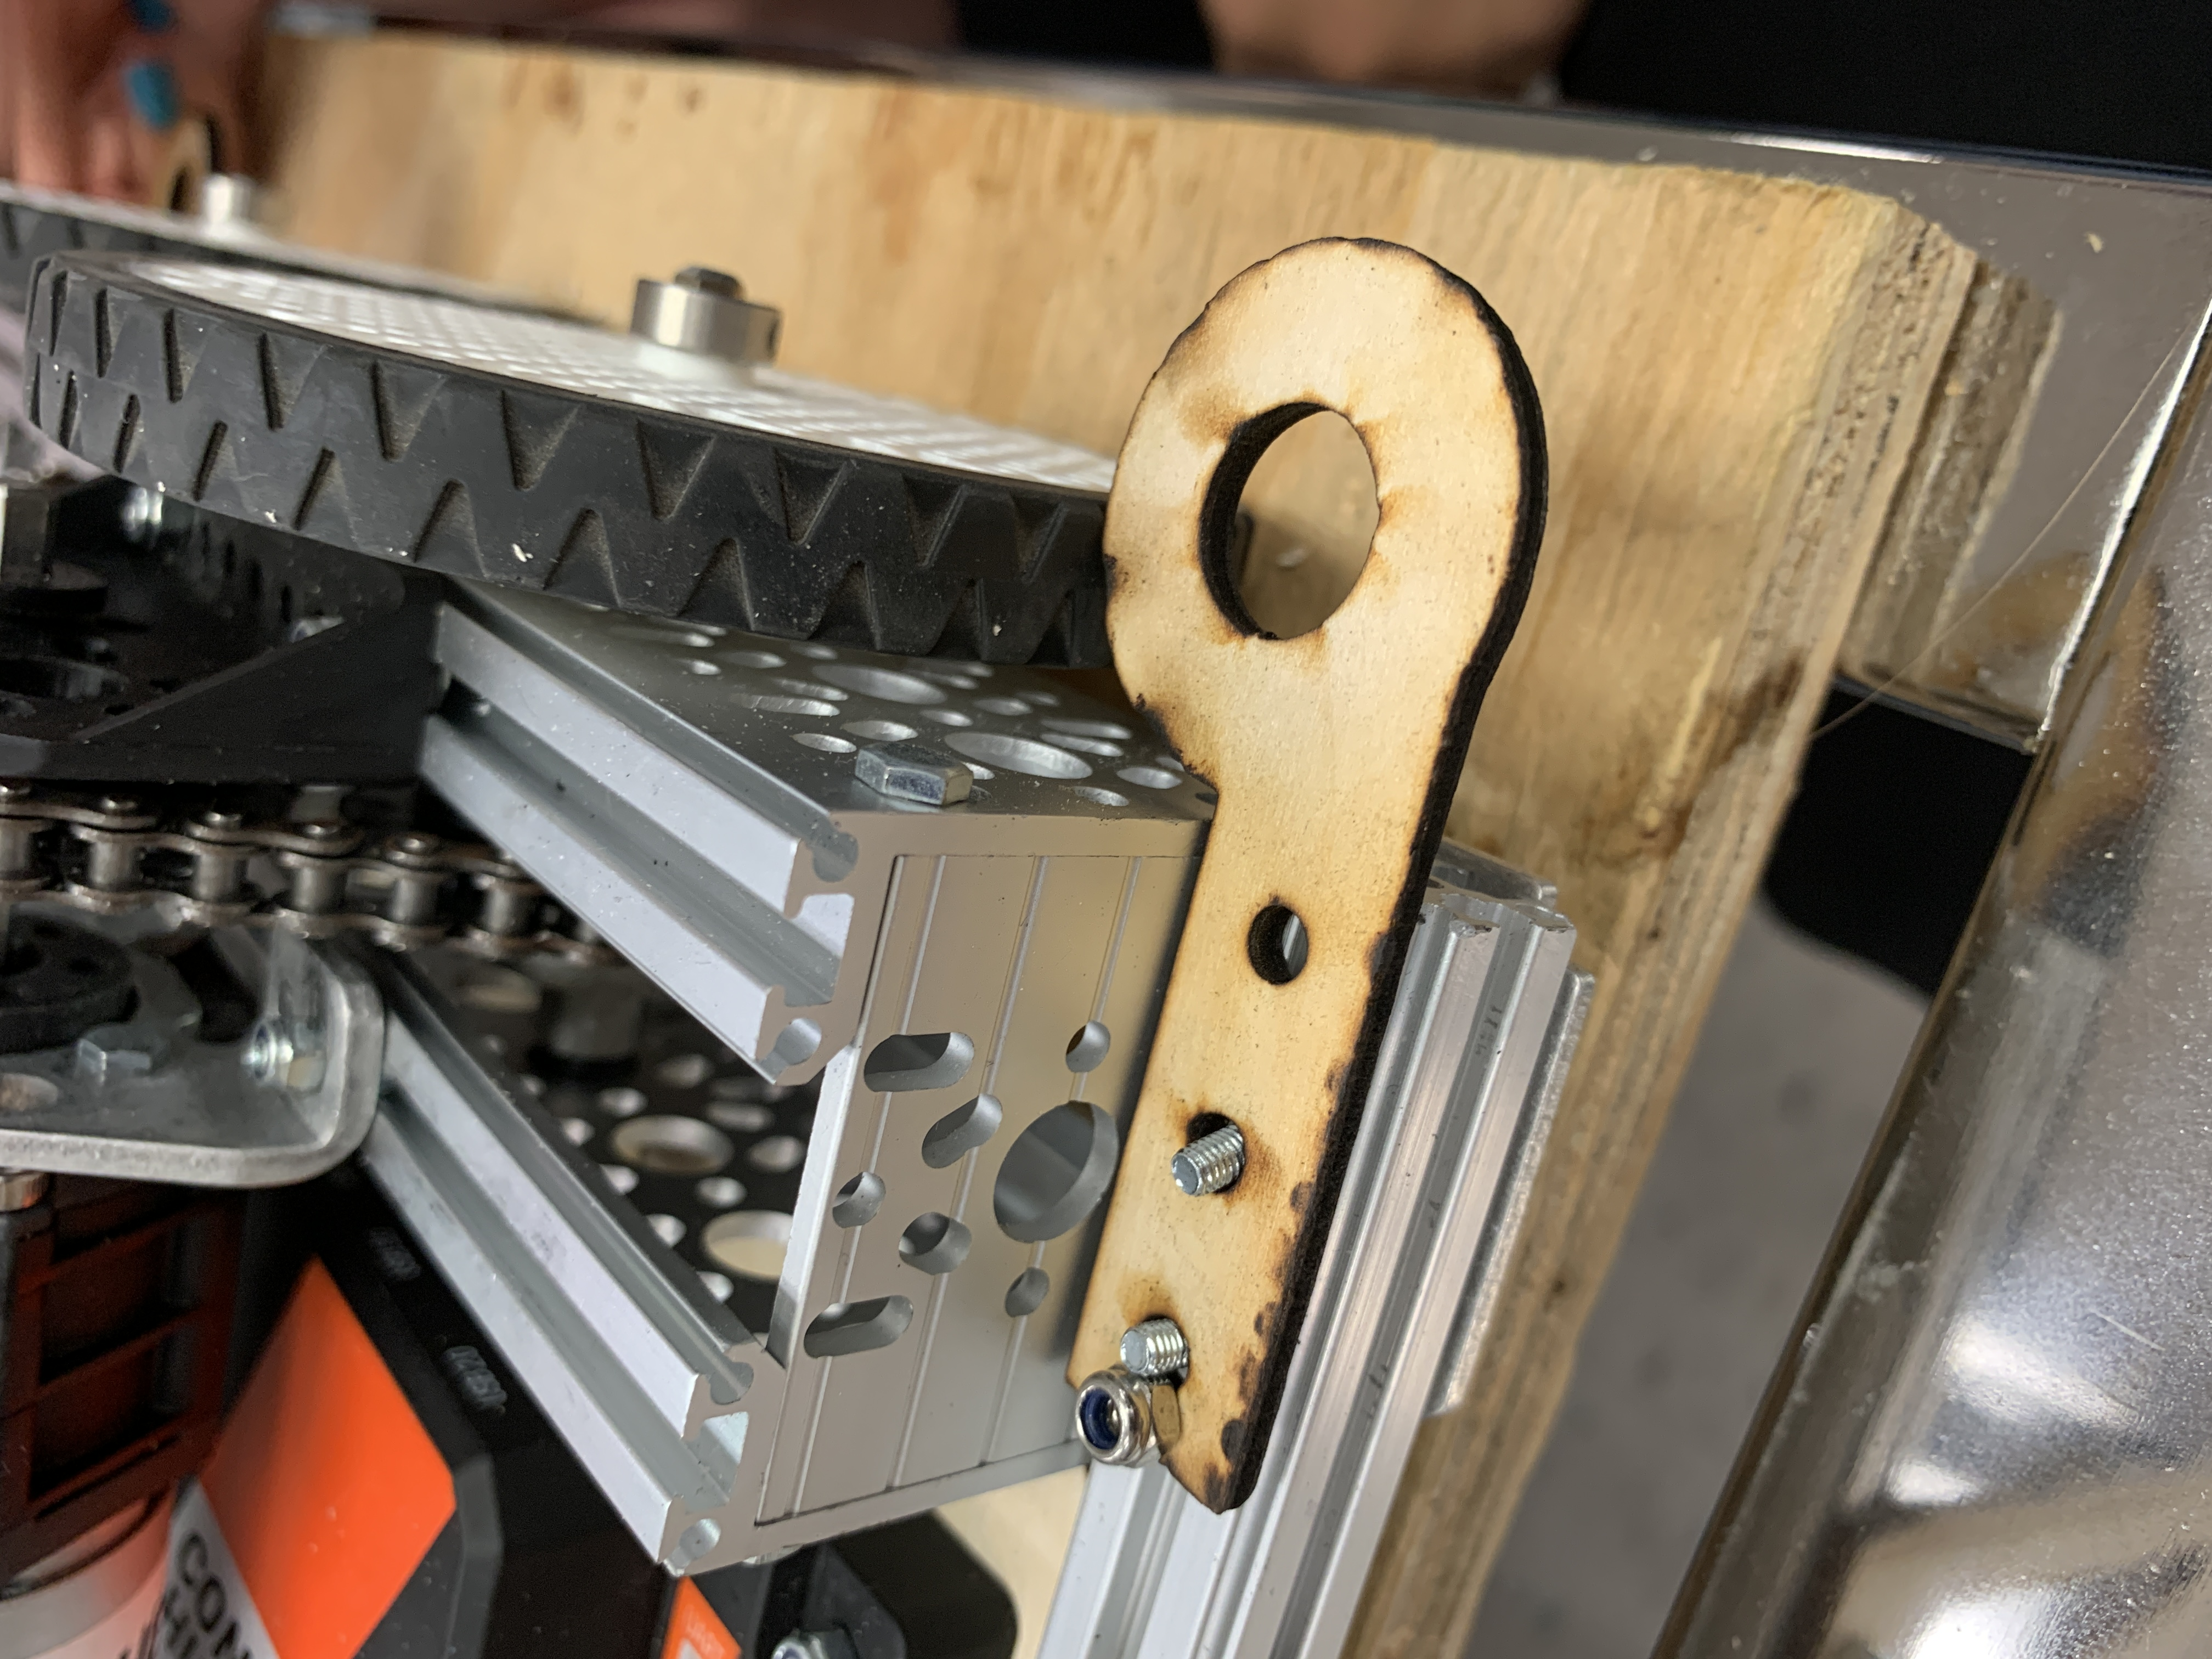
\includegraphics[width=0.8\textwidth]{Meetings/October/10-12-21/10-12-21_Team_Figure2 - Nathan Forrer.JPG}
  \caption{New rounded parts.}
  \label{fig:pic2}
\end{minipage}
\end{figure}

\begin{figure}[ht]
\centering
\begin{minipage}[b]{.50\textwidth}
  \centering
  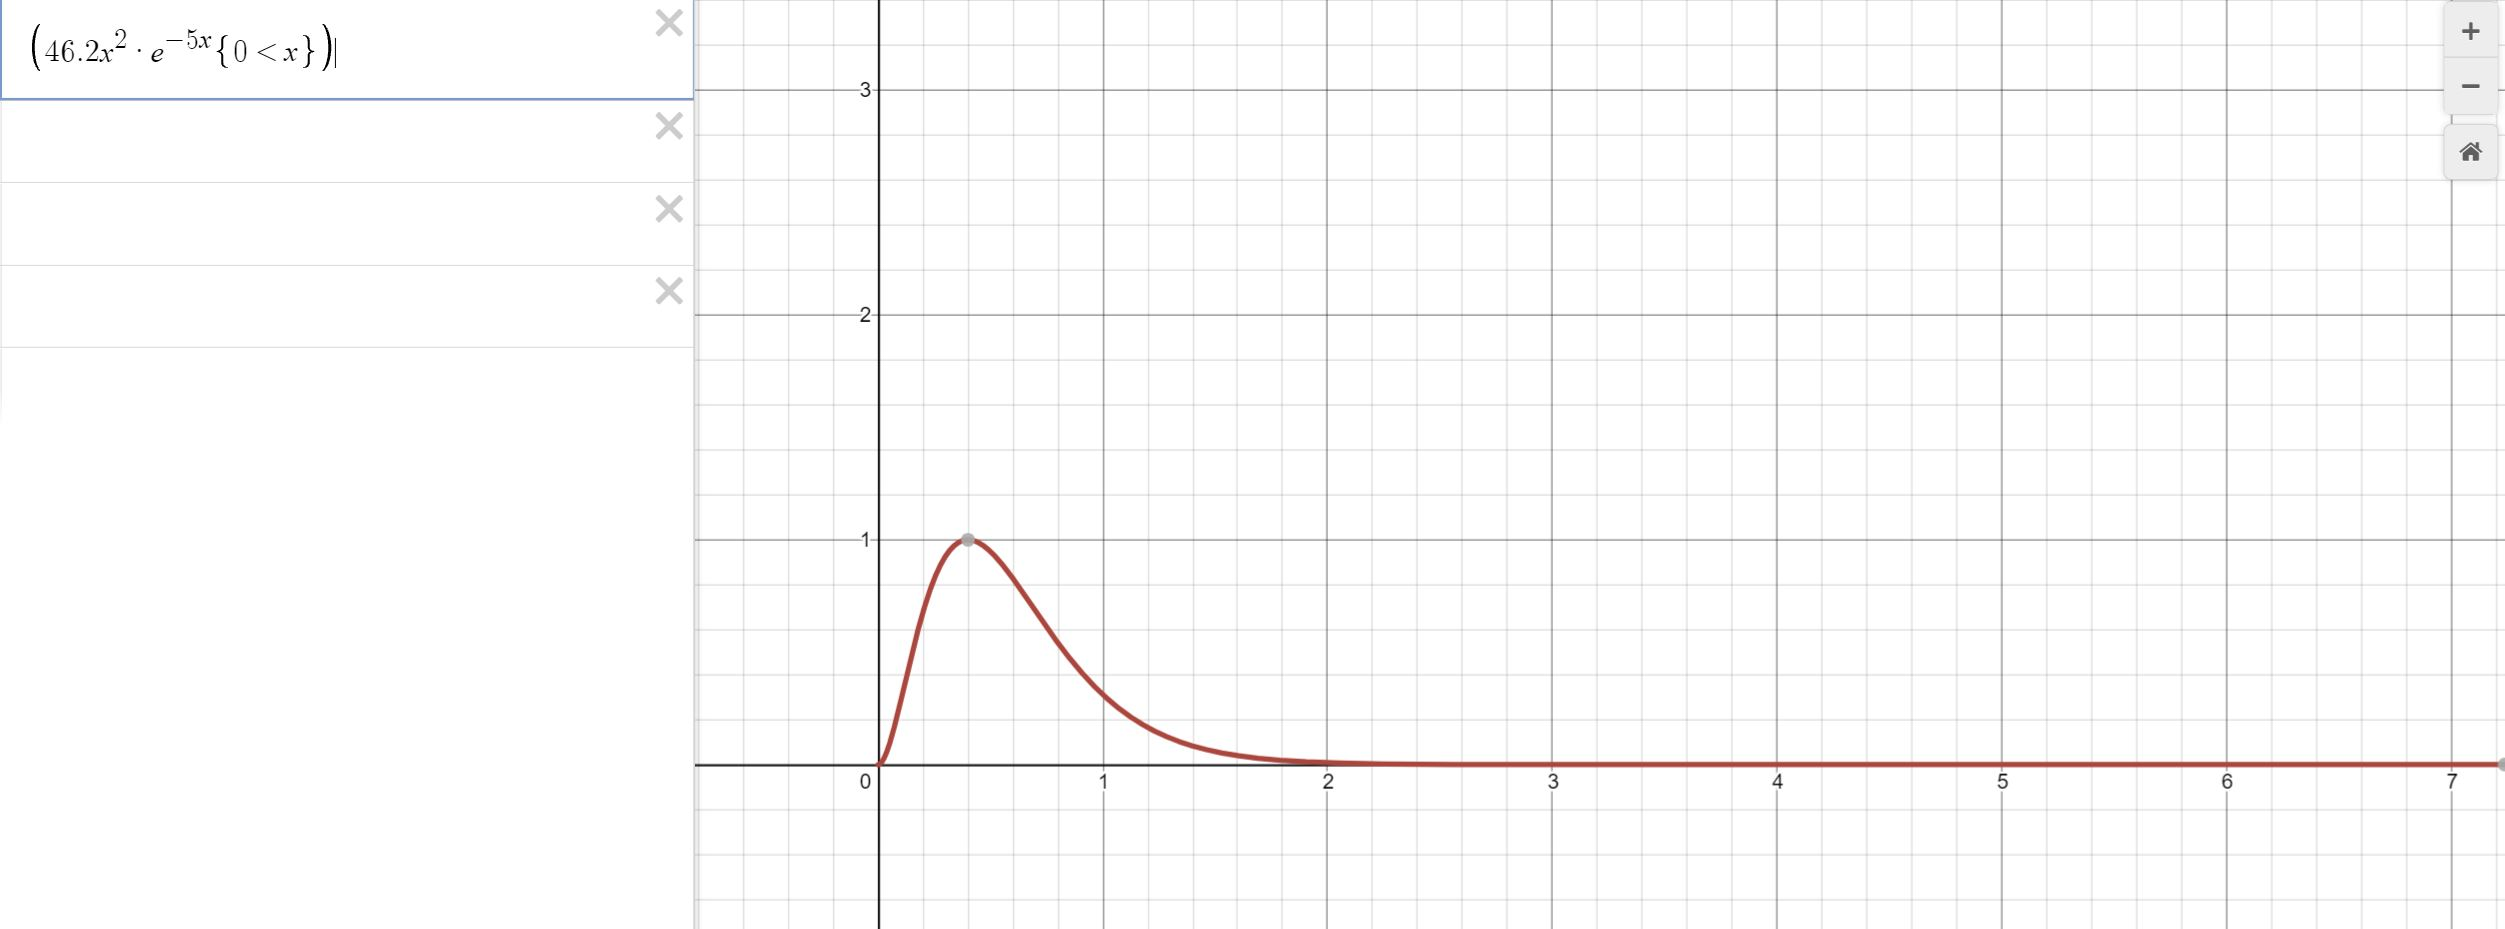
\includegraphics[width=0.8\textwidth]{Meetings/October/10-12-21/10-12-21_Team_Figure3 - Nathan Forrer.PNG}
  \caption{Equation for controlling the arm.}
  \label{fig:pic3}
\end{minipage}%
\hfill%
\begin{minipage}[b]{.50\textwidth}
  \centering
  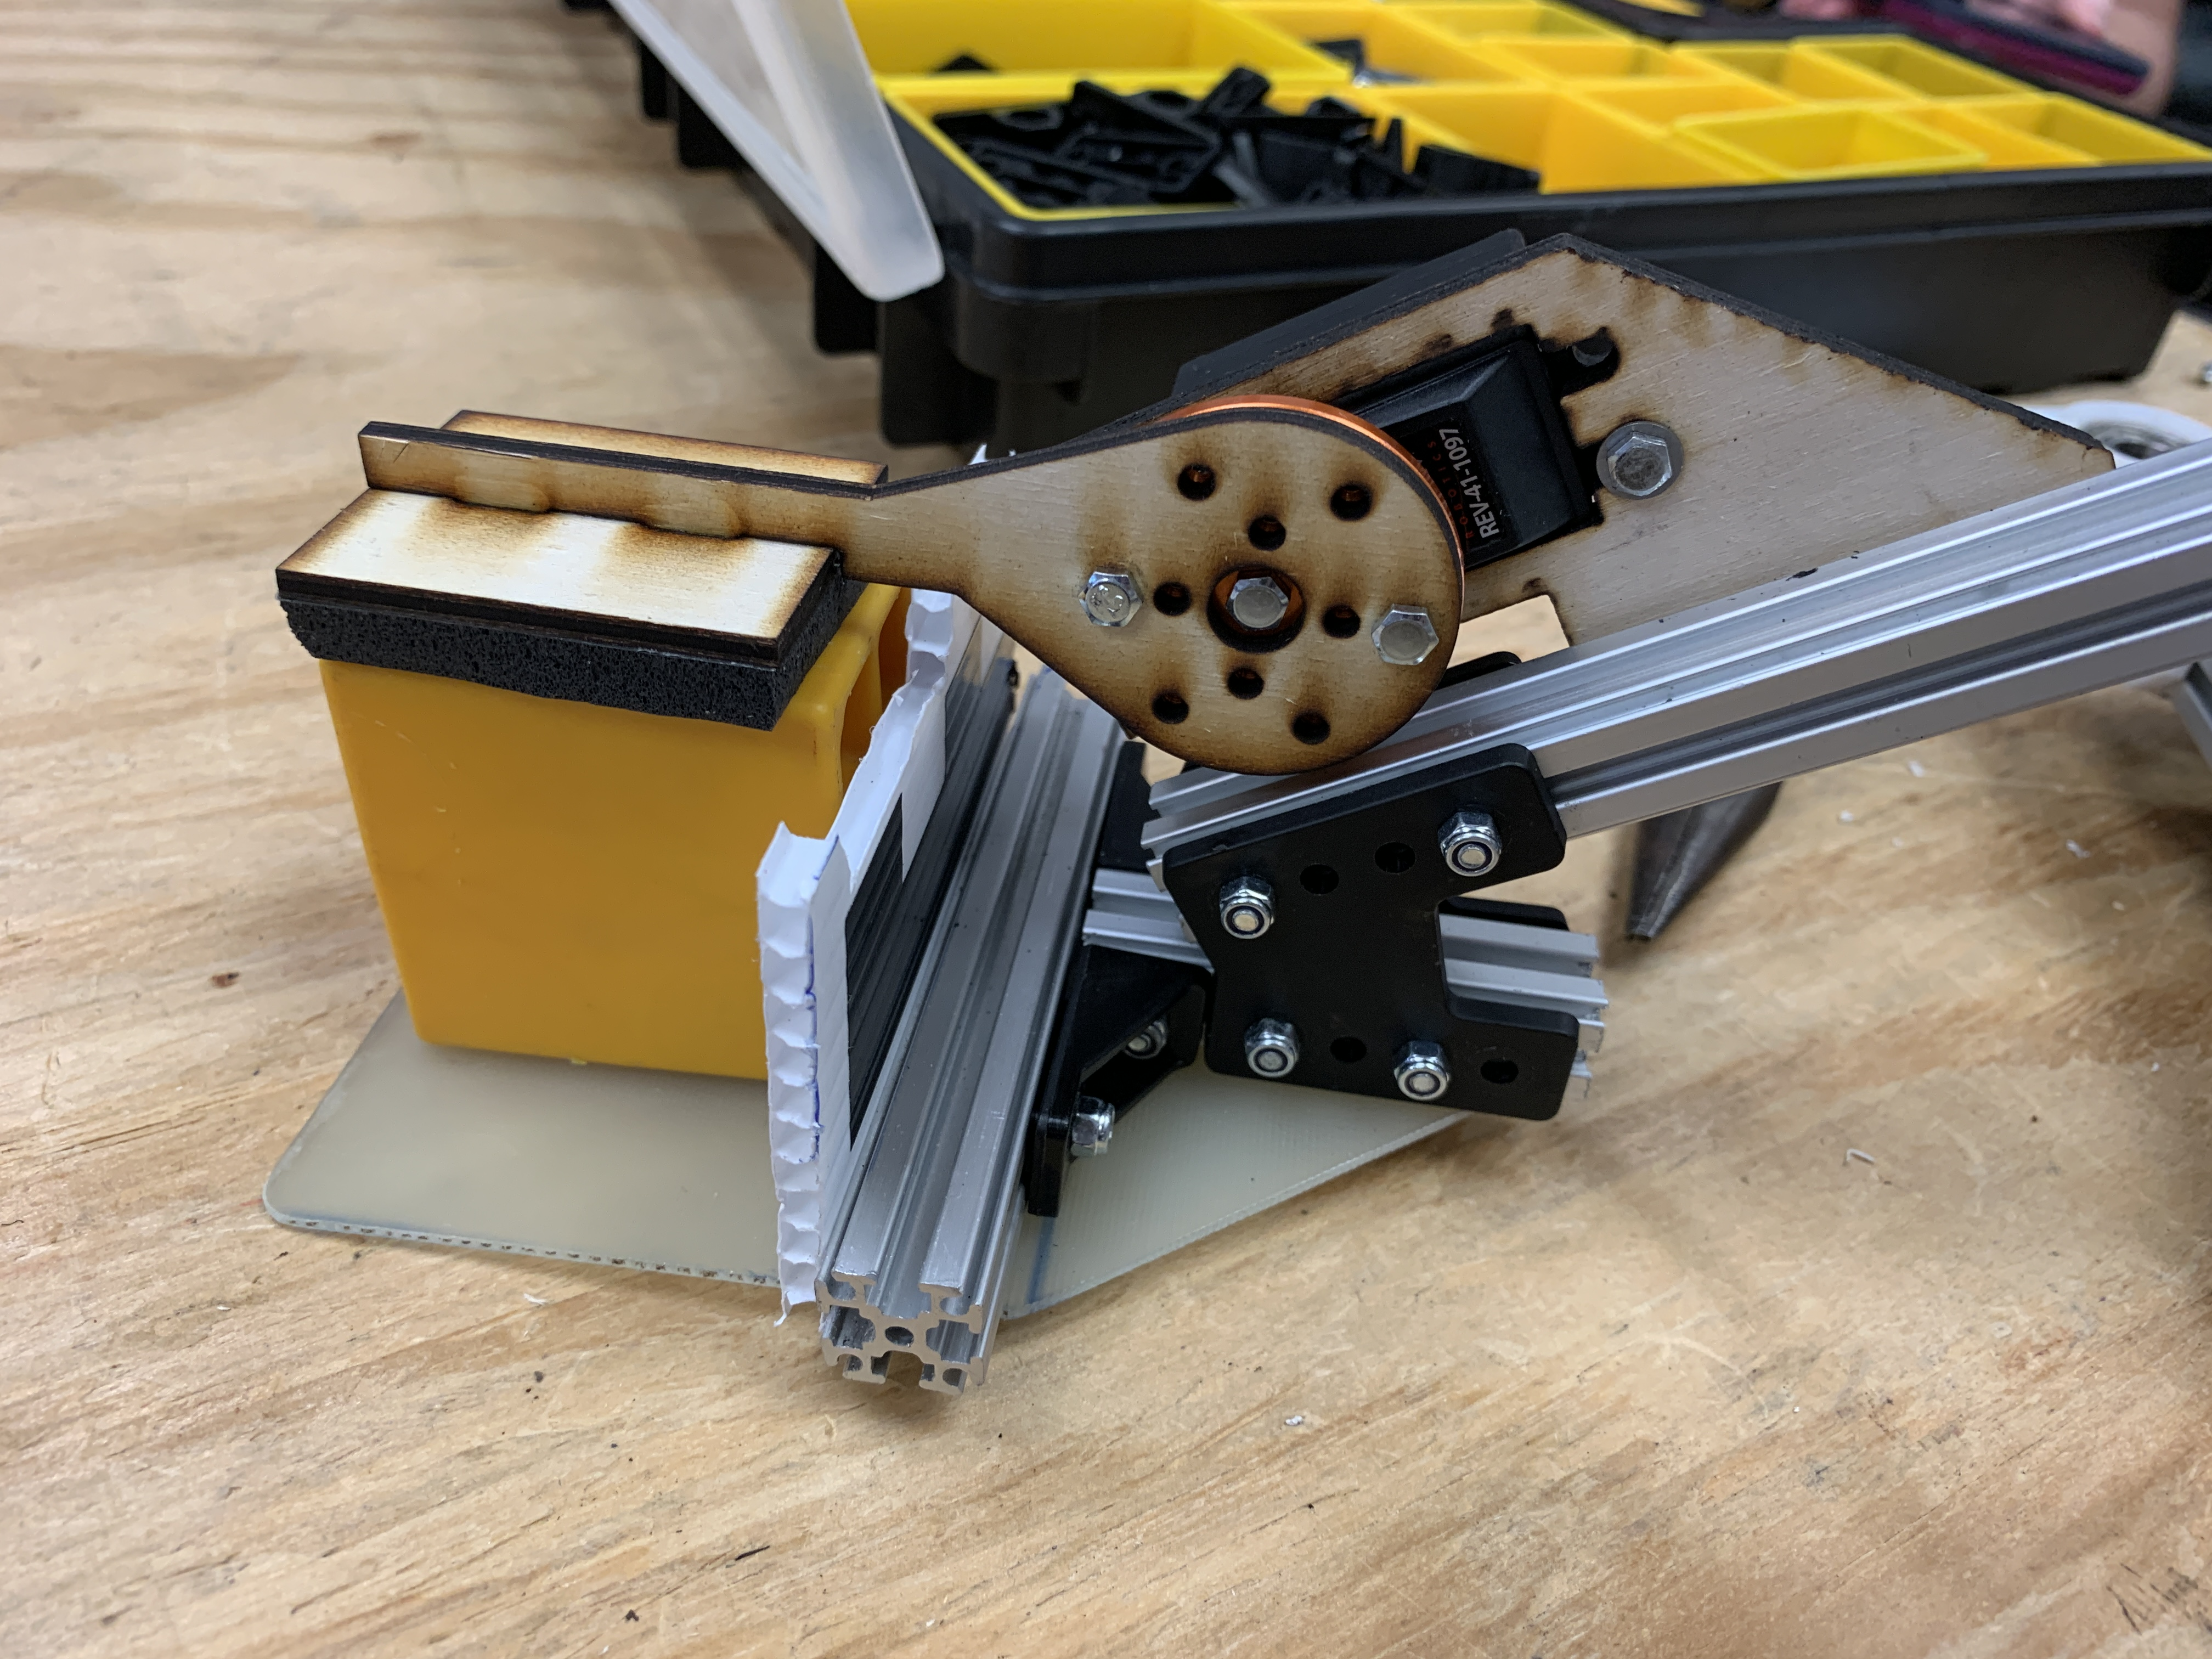
\includegraphics[width=0.8\textwidth]{Meetings/October/10-12-21/10-12-21_Team_Figure4 - Nathan Forrer.JPG}
  \caption{The grabber.}
  \label{fig:pic4}
\end{minipage}
\end{figure}